\section{Storage System}

The purpose of the storage system is to rotate a disk with 8 storage positions to a requested location, so that objects can be delivered to or retrieved by the UR robot arm. The storage disk is divided into eight positions, where each position corresponds to one storage slot.

The system consists of a circular disk, a geared DC motor, a laser-engraved encoder pattern, four light dependent resistors (LDRs), an external ADC, and a Raspberry Pi Pico for local control. The Pico receives target-position commands from the main PC and controls the motor until the requested storage position has been reached.

The disk is driven by a 24 V DC motor through a 6 mm timing belt and a 1:3 gear reduction. The gear reduction was implemented to reduce the rotational speed and increase the available torque, making the movement more suitable for controlled positioning.

\begin{figure}[H]
    \centering
    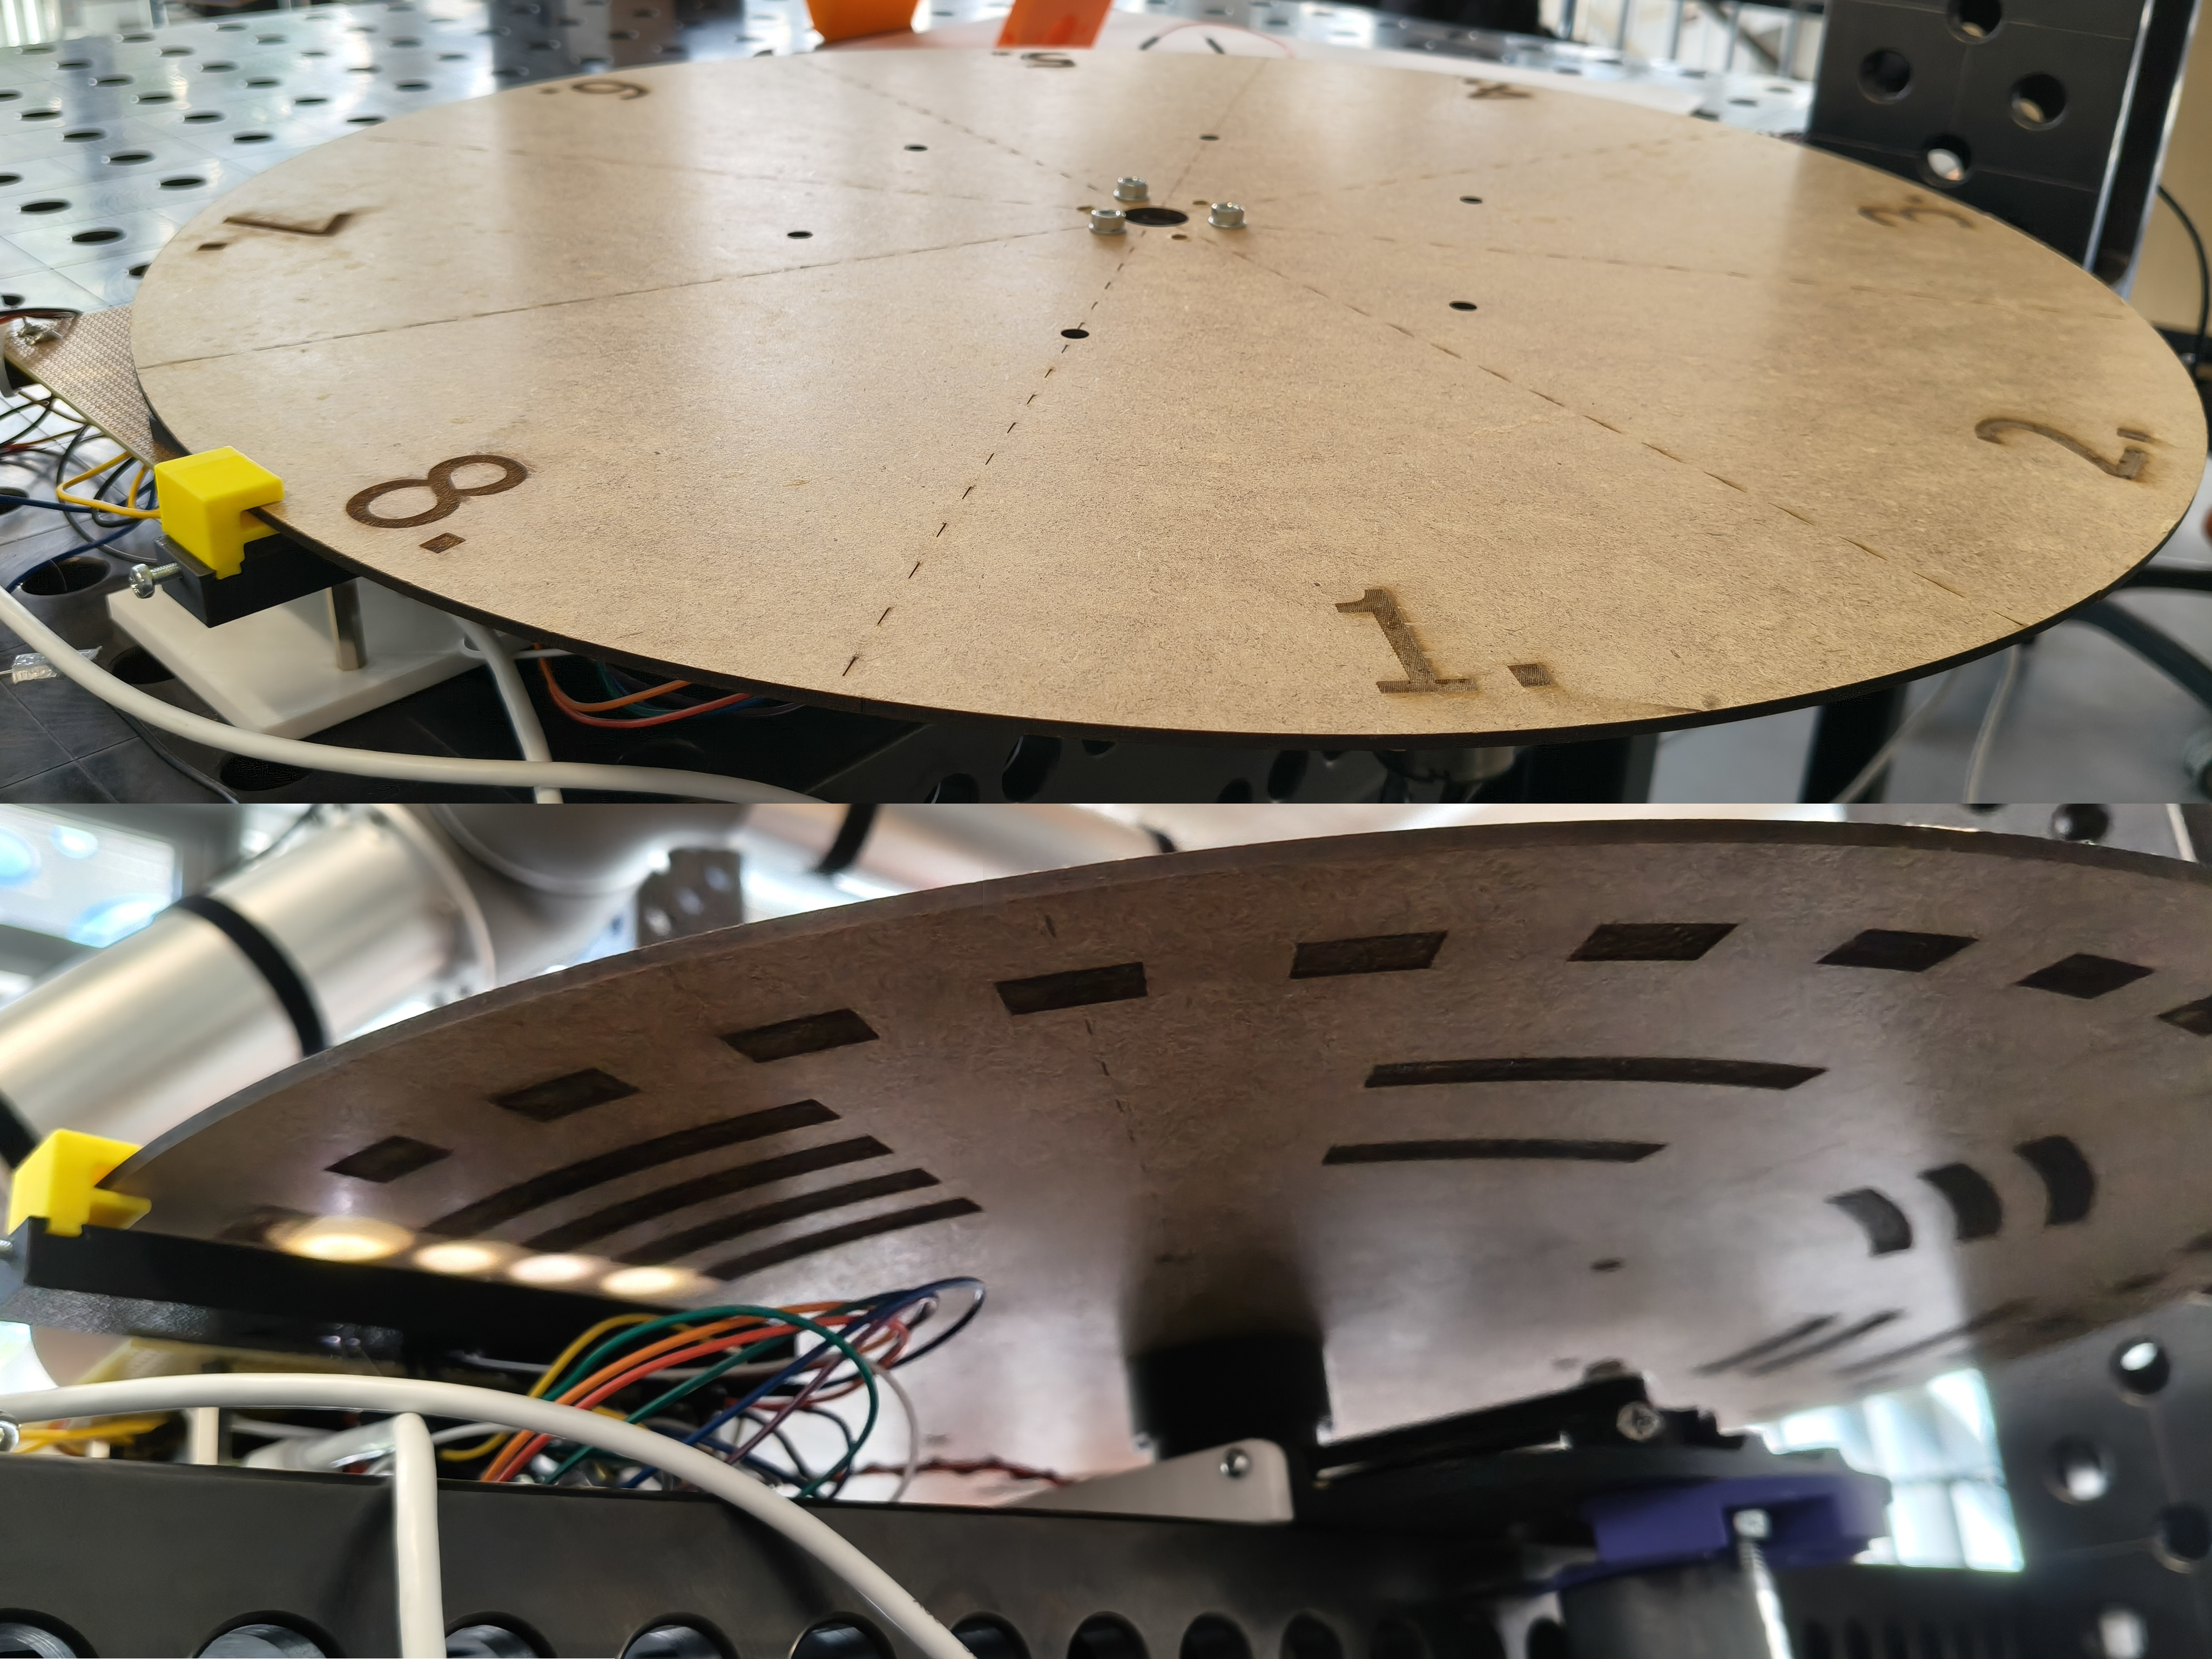
\includegraphics[width=0.7\textwidth]{figures/Semesterprojekt2SkiveBillede001v2.png}
    \caption{Storage disk with engraved storage positions.}
    \label{fig:storage-disk}
\end{figure}


%\subsection{System Control, Mechanical and Encoder Design}
%\subsection{Hardware and Local Control}
\subsection{Encoder Design and Local Control}

The storage disk uses a binary absolute encoder engraved on the underside of the disk. The encoder is read by four LDR sensors placed below the disk. Since the engraved and non-engraved areas reflect different amounts of light, the analog LDR readings can be converted into binary values.

Three of the encoder lanes are used for position encoding, giving $2^3=8$ possible position codes. The fourth lane is used as a control lane to verify that the sensors are currently reading a valid encoder area. This is necessary because the binary value \texttt{000} is a valid storage position. Without the control lane, the software would not be able to distinguish between a valid \texttt{000} position and the blank area between encoder markings.

The use of an absolute encoder means that the system does not need to count every transition while the disk rotates. Instead, the current position can be determined directly from the measured binary pattern. This was important because the storage system only needs to know which storage position is currently aligned with the robot, not the exact angular position of the disk at every moment.


An extra outer lane was originally included as a relative encoder lane, but it was not used in the final implementation. Reliable relative decoding would require every transition to be detected while the disk is moving. This was not suitable with the measured LDR response time and software loop time, as shown in Appendix~\ref{app:encoder-speed-calculations}. The absolute encoder was therefore chosen because each valid reading directly identifies the current storage position without depending on transition counting.

%Just remember to improve appendix :D
%An extra outer lane was originally included as a relative encoder lane. This lane was intended to detect repeated transitions during rotation. However, it was not used in the final implementation. A relative encoder depends on detecting every transition while the disk is moving, which makes it more sensitive to sensor response time and software loop time. Based on the LDR rise time of approximately 30 ms \cite{gl5528_datasheet}, and the $4.5^\circ$ encoder marking width, the theoretical maximum speed for reliable relative transition detection was calculated to approximately 12.5 RPM, Appendix~\ref{app:encoder-speed-calculations}. Practical testing showed an average software loop interval of approximately 38 ms even before LDR averaging was included, reducing the practical margin further. The absolute encoder was therefore more suitable, since it allowed the position to be determined directly from a valid bit pattern instead of relying on transition counting.

%A fifth outer lane was originally included as a relative encoder lane. This lane was intended to detect repeated transitions during rotation. However, it was not used in the final implementation. A relative encoder would require reliable detection of every transition while the disk is moving, which was difficult because of LDR response time, ADC sampling, and software loop time. The absolute encoder was sufficient, since it allowed the position to be determined directly from a valid bit pattern instead of relying on transition counting.


%REMEMBER TO ADD THE SOURCES FROM APPENDIX, SPECIFIC MOTOR, LDR, ADS!

%\subsection{Control Electronics}

%The storage system is controlled by a Raspberry Pi Pico. 
The Raspberry Pi Pico handles the local control, including encoder readings, position decoding, path calculation and motor control. The LDR signals are read through an external ADS7830 ADC\cite{ads7830_datasheet}, since four analog channels are required for the encoder.

At system level, the PC only sends target-position commands, \texttt{CMD GOTO <position>},to the Pico over UART, while the Pico performs the local movement and returns a response when the requested position has been reached. This follows the same general command-response structure as the gripper interface described in Section~\ref{sec:gripper-software}.

%locally while listening for commands over UART by the same logic as described in Section~\ref{sec:system-architecture} and as described in Section~\ref{sec:gripper-software}.

%
%Communication with the main PC is handled using a string-based command protocol over UART. This allows the main system to send target-position commands to the storage controller and receive acknowledgements when the movement is complete.

%Each LDR is connected in a voltage divider circuit, where the output voltage changes depending on the light level. An external ADS7830 ADC converts these voltages into digital values, which are then processed by the Pico. The built-in ADC of the Raspberry Pi Pico was not sufficient because the absolute encoder requires four analog channels, while the Pico only provides three usable ADC inputs.  

%HAr ændret lidt i det alexander, har gemt din tekst, hvis du ikke er enig med ændringerne.

%I had to cut it :C it is too much hardware, it like ofcourse we use a H-Bridge... 
%The disk is rotated using a 24 V DC motor controlled with a H-bridge driver. The H-bridge allows the motor to rotate in both directions, so the disk can move clockwise or counter-clockwise depending on the shortest path to the target position. PWM from the Pico is used to control the motor speed.

%In the final implementation PWM is constant


\subsection{Calibration and Encoder Interpretation}

The encoder thresholds are calibrated every time the system starts. This is necessary because LDR readings are affected by ambient lighting, sensor placement, and reflection from the disk surface. A fixed threshold would therefore not be reliable under all test conditions.

%The calibration is performed by aligning the disk with storage position 4, where all four absolute encoder LDRs are engaged 4. A custom conversion was used for no reason at all is [1111] the full Ciffer-Table is avaiable in the appendix. The disk is then moved so that both high and low readings can be collected from each sensor. The calibration sequence is shown in Figure~\ref{fig:ldr-calibration-data}.

Calibration is performed by first aligning the disk with storage position 4, where all four absolute encoder LDRs are active. This gives the reference bit pattern \texttt{1111}. The full encoder conversion table is provided in Appendix~\ref{app:ciffertabel}. The disk is then moved so that each LDR records both engraved and clear areas of its encoder lane, allowing individual thresholds to be calculated. The calibration sequence is shown in Figure~\ref{fig:ldr-calibration-data}.


\begin{figure}[H]
    \centering
    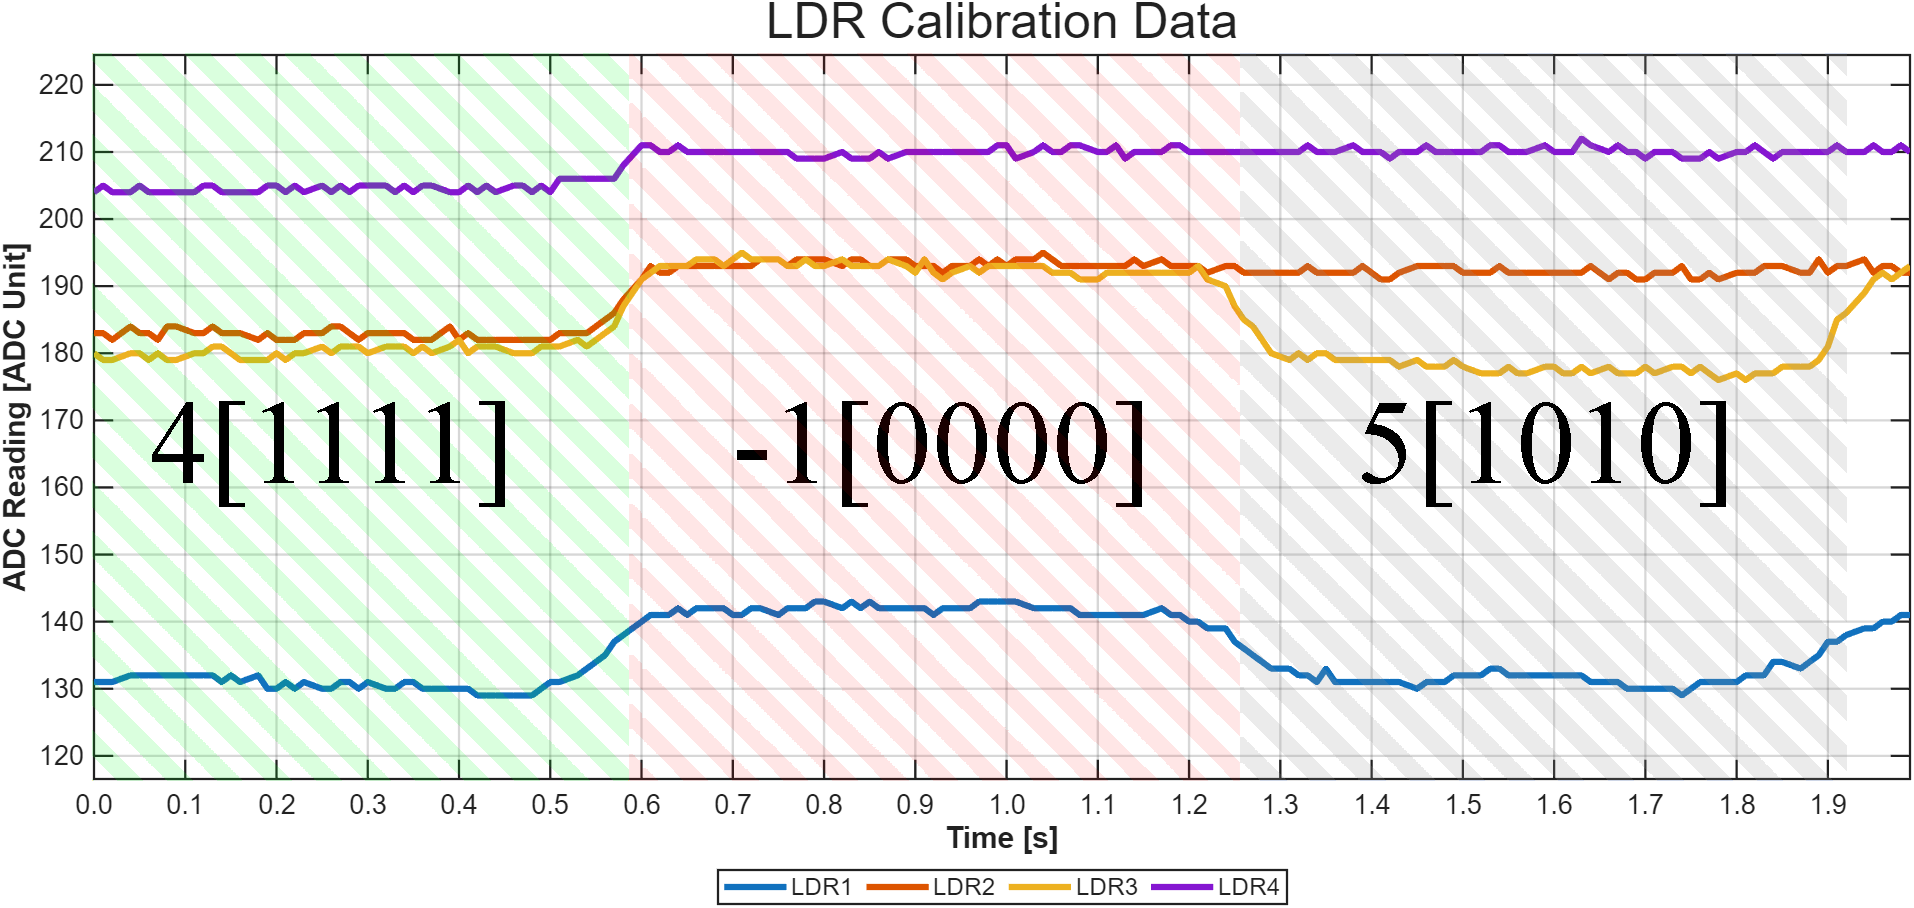
\includegraphics[width=0.9\textwidth]{figures/LDRCalibrationDatasemester2_skraveretV2.png}
    \caption{LDR calibration data.}
    \label{fig:ldr-calibration-data}
\end{figure}

After the calibration data has been collected, the highest and lowest 20\% of the measured values are used to calculate the threshold for each LDR. The average of the lower range and the average of the upper range are found, and the threshold is placed between them. Values above the threshold are interpreted as binary 0, while values below the threshold are interpreted as binary 1.

During normal operation, each LDR value is read several times and averaged before being converted into a binary value. In the tested implementation, each reading is based on five ADC samples. This reduces the influence of individual noisy measurements and makes the binary interpretation more stable.

The decoder combines the four binary LDR values into one encoder reading. The three position lanes are compared with a lookup table, where each valid bit pattern corresponds to one of the eight storage positions. The fourth lane is used to determine whether the reading is valid. If the measured pattern does not correspond to a valid encoder state, the decoder rejects the reading and returns \texttt{-1}. This invalid state can be seen in the calibration data in Figure~\ref{fig:ldr-calibration-data}, where the sensors pass through an area between valid encoder markings.

% as seen in Figure~\ref{fig:ldr-calibration-data}.

The processed encoder signal is shown in Figure~\ref{fig:encoder-signal-processing}, where the analog LDR reading is converted into a binary signal.

\begin{figure}[H]
    \centering
    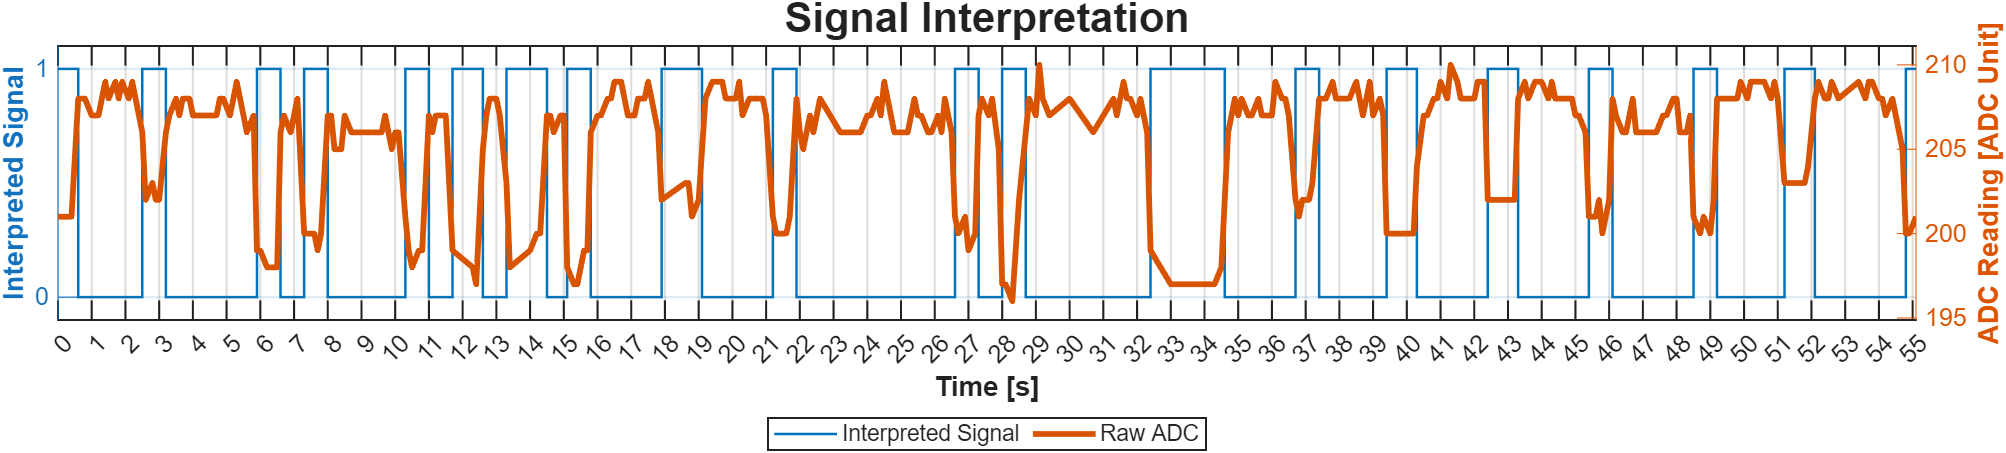
\includegraphics[width=1\textwidth]{figures/Signal Interpretation_corrected.png}
    \caption{Processed encoder signal.}
    \label{fig:encoder-signal-processing}
\end{figure}

%evaluation in title?
%\subsection{Control Software and Performance Improvements}
%\subsection{Performance improvements and Evaluation}
\subsection{Encoder Software Improvements}

The storage system software was divided into smaller classes to separate motor control, encoder reading, decoding, route calculation, and data logging. This made the system easier to test, because individual parts of the control loop could be changed without rewriting the full program.

The DC motor class controls the motor direction through two digital output pins and controls the enable signal using PWM. The motor can therefore be driven forwards, backwards, or stopped depending on the calculated direction of travel.

The pathfinder class determines the shortest rotational path between the current position and the requested target position. Since the disk has eight positions arranged in a circle, the shortest path may cross the transition between position 8 and position 1. For example, if the current position is 2 and the target position is 8, the shortest movement is two positions in the negative direction rather than six positions in the positive direction. The route calculation therefore returns both the required distance and the direction of travel.



A major challenge during testing was that the encoder could produce incorrect intermediate readings while the disk was moving. This happened because the four LDR readings had a small delay between each LDR when averaging values. If the disk moved between individual sensor readings, the software could combine values from slightly different physical positions and interpret them as one incorrect bit pattern.

%Abnormality in flow here...

%interval between readings instead of loop time

This was supported by timing measurements of the reading loop. When only raw LDR values were read, the average loop time was approximately 38 ms after subtracting the intentional \texttt{sleep\_ms} delay. Since normal operation also used averaging of five ADC samples per LDR, the full encoder reading loop was slower than the theoretical LDR response time alone would suggest. The problem was therefore not only the sensor hardware, but the combined timing of sensor response, ADC communication, averaging, and software execution.

To reduce this error, the LDR reading function was changed so that the four sensor values were treated as one synchronized encoder sample. This made the decoder less likely to combine old and new sensor states into a false position reading.

A second improvement was expected-position decoding. Since the software knows both the current position and the direction of movement, it can predict which encoder position should appear next. The decoder can therefore reject readings that may be valid binary patterns in isolation, but are impossible in the current movement sequence. For example, if the disk is moving from position 4 toward position 3, a sudden reading of position 8 can be rejected as an invalid transition.

%Herefter er det data

%Herefter er det data

%Herefter er det data

\subsection{Positioning Performance Evaluation}


The effect of the software changes was evaluated by comparing repeated test runs with different encoder configurations. For each configuration, the system was tested six times, with each test lasting five minutes. A deterministic sequence of randomly selected target positions was used by seeding the random number generator with the same value for each test. This ensured that each configuration was tested under comparable conditions.

During each test, the measured encoder positions were logged and compared with the expected position sequence. An irregularity was counted when the measured sequence skipped one or more expected positions. For example, the sequence \texttt{1, 2, 3, 4} was considered valid, while \texttt{1, 2, 4} contained one irregularity because position 3 was skipped.

Encoder performance was evaluated using three parameters: average task time, irregularity rate, and standard deviation of irregularity rate. The average task time indicates how quickly the system reached the requested target positions. The irregularity rate was used as the main indicator of reading accuracy, since it describes how often the measured encoder sequence deviated from the expected sequence. The standard deviation between the six repeated tests was used to evaluate consistency, since it shows how repeatable the results were for each configuration.

Both reading accuracy and consistency are important for the storage system. A system that occasionally works correctly but gives highly variable results is difficult to trust. Likewise, a system that behaves consistently but produces incorrect readings is still undesirable. The best configuration is therefore the one that combines a low irregularity rate with low variation between repeated tests, while still maintaining an acceptable task time.

%The effect of these software changes were evaluated by comparing repeated test runs with different configurations. A deterministic target sequence was used so that each configuration was tested under comparable conditions. An irregularity was counted when the measured position sequence skipped one or more expected positions. 

%Each implementation was tested six times for 5 minutes each. During each test, the measured encoder positions were logged and compared with the expected sequence.

%The encoder performance was evaluated using task speed, reading precision, and reading consistency. Reading precision describes how well the measured sequence matches the expected sequence. Reading consistency describes how repeatable the results are between repeated test runs.

%The rate of irregularities relative to successfully finding the requested target was used as the primary indicator of precicion. The standard deviation between repeated test runs was used to evaluate consistency.

%For each implementation and data gathering, the system were adjusted with the specified set of parameters and implementations and set to run for 5 minutes with a deterministic set of randomly selected targets using the srand function, this was repeated 5 times for a total of 6 readings per implementation, here the number of inaccuracies in the order of readings is an indicator of precicion, and the standart deviation between the 6 tests indicates the accuracy of the system.

%Both are vital, consistency because if you cannot replicate your results, then how can you ever know what to expect, how is the system better than chance. This is usually the most important trait to focus on, however if you can consistently get 0 successive reading, the precision is low and the system is still not usefull.

%Consistency (accuracy) std deviation in samples, if the system can consistently reach the same target

%Precision: how well does what we read actually match what we should read.

%Improved table

\begin{table}[H]
\centering
\small
\begin{tabular}{|c|c|c|c|}
\hline
Configuration & Avg. task time [s] & Irregularity rate & Irregularity std. dev. \\
\hline
None & 3.5 & 99\% & 25\% \\
Sync. LDR reading & 3.2 & 16\% & 7\% \\
Expected-position decoding & 3.4 & 15\% & 4\% \\
Both & 3.3 & 13\% & 5\% \\
\hline
\end{tabular}
\caption{Encoder performance with different software implementations.}
\label{tab:encoder-software-performance}
\end{table}

%The results are placed in Appendix~\ref{tab:encoder-performance-software}.

%The tests showed that encoder reliability was improved through software implementations, but that either one was able to substantially improve the system precicion and accuracy, that both software implementations together provided the best results but that the expect next reading implementation has the most noticeable effect.

%The test results show that the encoder reliability was improved by the added software implementations. Both synchronized LDR reading and expected-position decoding reduced the irregularity rate substantially as well as decreasing inconsistency between each test compared with the original implementation.
%The irregularity rate of 99\% in the original implementation does not mean that 99\% of storage operations failed, but the skipped or unexpected encoder transitions occured frequenltly during movement.
%The best result was achieved when both implementations were used together, although the expected-position decoding had the most noticeable individual effect. This indicates that many of the encoder errors were not caused by the sensor readings alone, but by how the measured bit patterns were interpreted during movement.

The test results show that encoder reliability was improved by the added software implementations. Both synchronized LDR reading and expected-position decoding substantially reduced the irregularity rate and improved the consistency of the results compared with the original implementation.

The irregularity rate of 99\% in the original implementation does not mean that 99\% of storage operations failed. Instead, it means that skipped or unexpected encoder transitions occurred frequently during movement.

The best result was achieved when both implementations were used together, decrease irregularity rate from 99\% to 13\% and generated more consistent result, decrease standart deviation of irregularity rate from 25\% to 5\% , see table \ref{tab:encoder-software-performance}

Expected-position decoding had the most noticeable individual effect. This indicates that many of the encoder errors were not caused by the sensor readings alone, but by the interpretation of the measured bit patterns during movement.

%remove from appendix as well if not mentioned
%Additional tests showed that running the UR robot nearby did not measurably affect encoder performance, 

%indicating that electromagnetic interference from the robot was not a source of error, apppendix Table~\ref{tab:encoder-performance-ur}.

%Extra lighting also did not improve the result beyond statistical uncertainty, Appendix~\ref{app:extra-data-collection} Table \ref{tab:encoder-performance-lighting}

%This suggests that the main limitation was not the general light level, but the consistency of the sensor readings and the timing of the software loop.

The PWM tests showed that lowering the motor speed by decreasing PWM from 95\% to 5\% could improve encoder reliability, but at the cost of longer average task time, Appendix~\ref{app:extra-data-collection} Table \ref{tab:encoder-performance-pwm}.
This agrees with the timing analysis in Appendix~\ref{app:encoder-speed-calculations}, since lower disk speed gives the LDRs and software loop more time to capture each encoder marking. The lowest PWM level gave fewer irregularities, but increased the average task time substantially. The final implementation therefore uses 95\% PWM, since it provided the best compromise between task speed, repeatability, and reading accuracy for the complete storage task.
%Then you have evalution of PWM, not just Encoder!
%maybe just cut this part?

%The PWM tests showed that lowering the motor speed could improve reliability, but at the cost of longer task time, appendix Table~\ref{tab:encoder-performance-software}. A very low PWM level gave fewer irregularities, but also increased the average task time substantiually. The final implementation uses high PWM since it still displayed the best ratio between task speed, consistency and precicion.


\subsection{Finale Implementation}


%We do not hae data or calculations to support this
%The encoder reliability was limited by the combined response time of the LDRs, ADC communication, and software execution time. Although the motor and gear reduction allowed the disk to rotate mechanically, reliable decoding required the disk to move slowly enough for each encoder marking to be sampled consistently.

%This limitation was one of the reasons the relative encoder lane was not used. A relative encoder depends on detecting every transition while the disk is moving. Missing a transition would cause the calculated position to drift. The absolute encoder was more robust for this application because each valid reading directly identifies the current storage position.

%The final storage system therefore uses the four-lane absolute encoder, startup calibration, averaged LDR readings, synchronized encoder sampling, and expected-position decoding. These choices made the system more reliable without requiring additional hardware. The most important improvement was not the raw sensor data itself, but how the software interpreted the sensor data during movement.

The final storage system therefore uses the three-bit absolute encoder with an additional validity lane, startup calibration, averaged LDR readings, synchronized encoder sampling, and expected-position decoding. These choices made the system more reliable without requiring additional hardware. The most important improvement was not the raw sensor data itself, but how the software interpreted the sensor data during movement.

%Further improvements could include optimizing the software loop time, improving the mechanical alignment between the disk and LDRs, adding blocking screen from ambient lighting, using faster optical sensors, or replacing the LDR-based encoder with a sensor type better suited for high-speed transition detection. However, the implemented solution was considered sufficient for the current project requirements, since the disk could reliably identify storage positions.
%without adding additional mechanical or electrical complexity.


%I am a little baffled that it ended on the wrong position, that wil perhaps have to be adressed in perspektive!